%
% randdef.tex
%
% (c) 2021 Prof Dr Andreas Müller, OST Ostschweizer Fachhochschule
%
\documentclass[tikz]{standalone}
\usepackage{times}
\usepackage{amsmath}
\usepackage{txfonts}
\usepackage[utf8]{inputenc}
\usepackage{graphics}
\usetikzlibrary{arrows,intersections,math}
\usepackage{ifthen}
\begin{document}

\newboolean{showgrid}
\setboolean{showgrid}{false}
\def\breite{7}
\def\hoehe{4}

\begin{tikzpicture}[>=latex,thick]

% Povray Bild
\node at (-3.8,0) {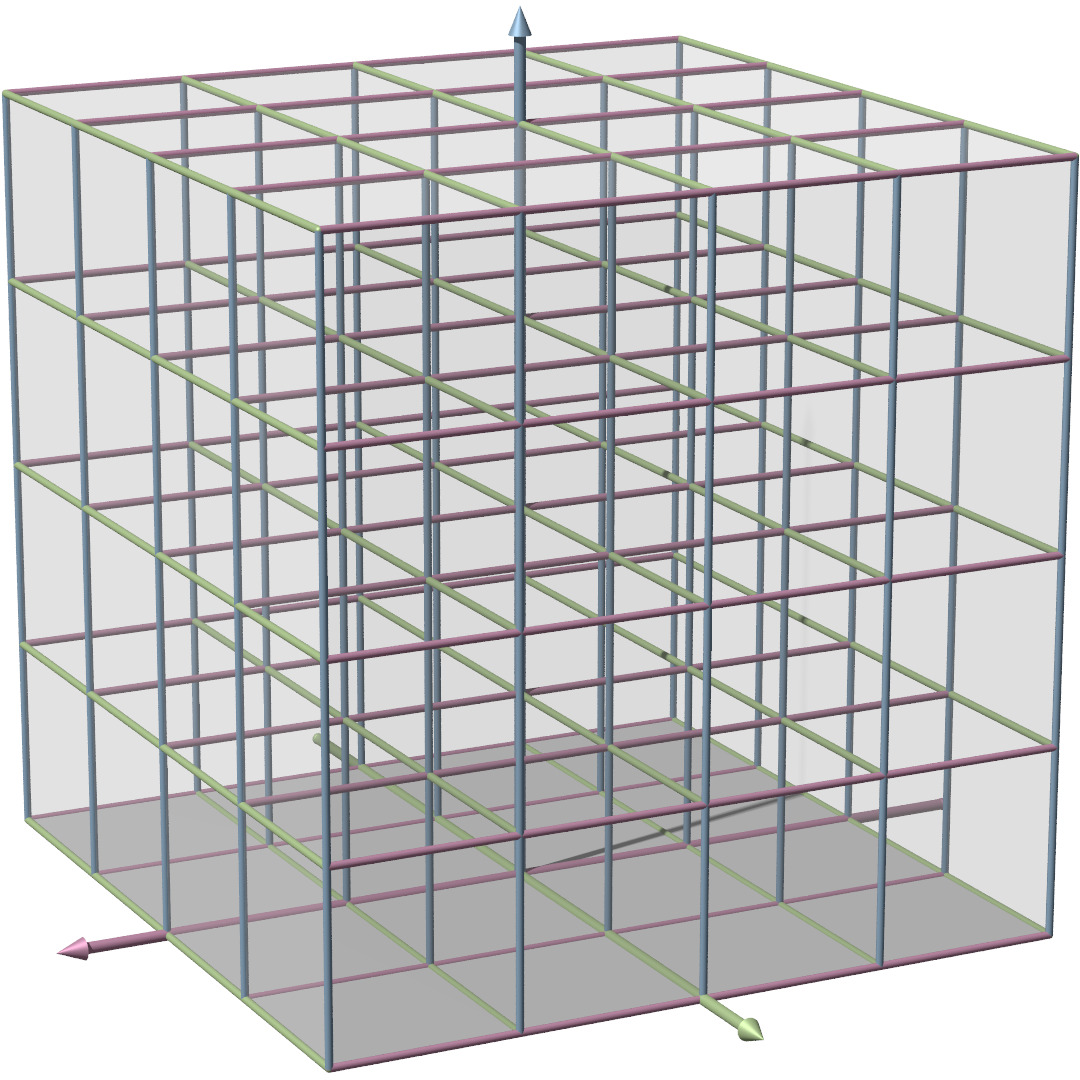
\includegraphics[width=4.4cm]{domain.jpg}};
\node at (3.3,0) {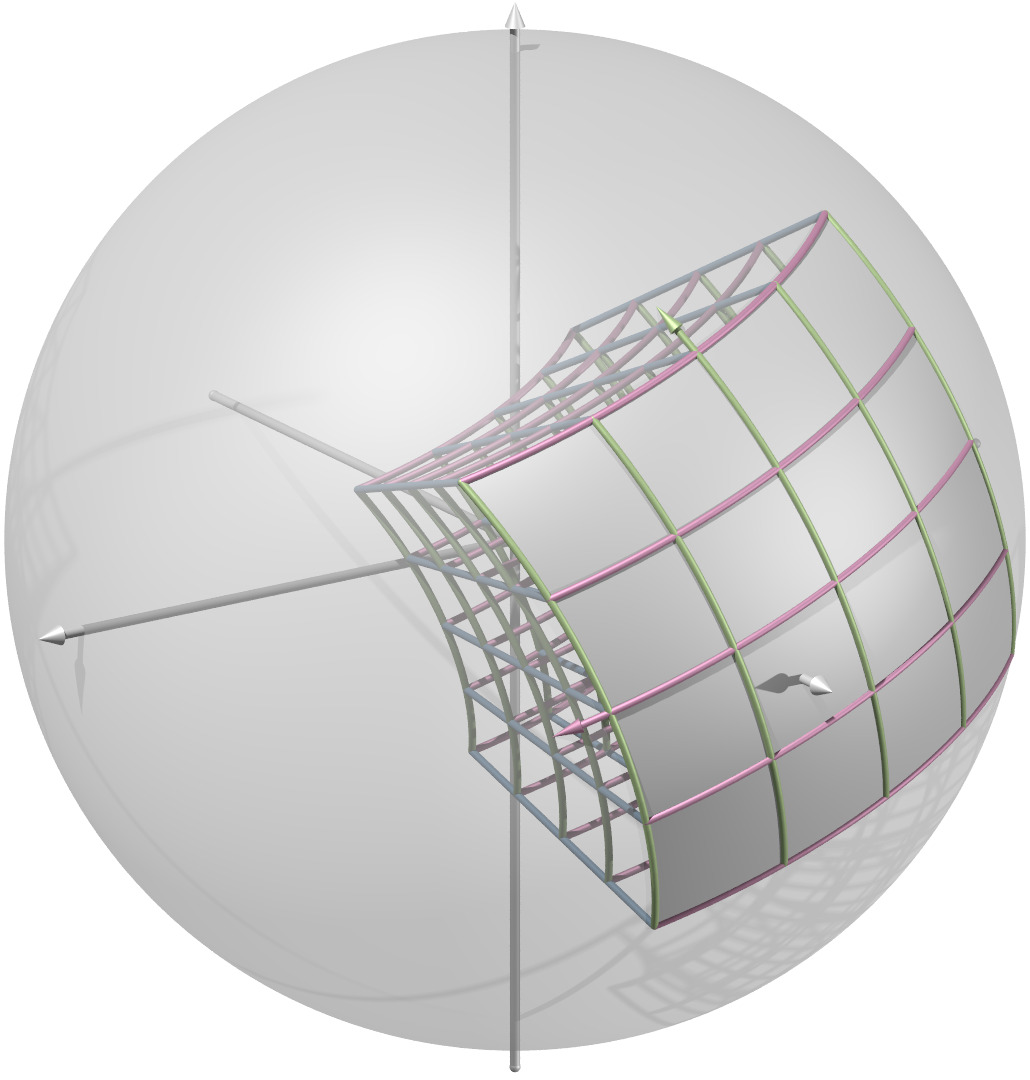
\includegraphics[width=6.0cm]{sphere.jpg}};

% Gitter
\ifthenelse{\boolean{showgrid}}{
\draw[step=0.1,line width=0.1pt] (-\breite,-\hoehe) grid (\breite, \hoehe);
\draw[step=0.5,line width=0.4pt] (-\breite,-\hoehe) grid (\breite, \hoehe);
\draw                            (-\breite,-\hoehe) grid (\breite, \hoehe);
\fill (0,0) circle[radius=0.05];
}{}

\node at (-5.9,-1.4) {$x_1\mathstrut$};
\node at (-2.7,-2.2) {$x_2\mathstrut$};
\node at (-3.7,2.3) {$x_3\mathstrut$};
\node at (-4.0,-3) [left] {$x_3=0\mathstrut$};
\draw[->] (-4,-3) to[out=0,in=-90] (-4,-2.1);

\node at (3.4,-1.2) {$x_1\mathstrut$};
\node at (4.0,1.5) {$x_2\mathstrut$};
\node at (4.7,-0.1) {$x_3=0\mathstrut$};

\draw[<-] (3.3,1.3) arc(60:110:6);
\node at (0.4,2.2) [above] {$\varphi\mathstrut$};

\end{tikzpicture}

\end{document}

